\documentclass[12pt]{article}
\usepackage{graphicx}
\usepackage{hyperref}
\usepackage{geometry}
\usepackage{float}
\usepackage{multirow}
\geometry{a4paper, margin=1in}

\title{Progress Report: LAI Estimation using 3D Gaussian Splatting vs. Terrestrial Laser Scanning}
\author{}
\date{\today}

\begin{document}

\maketitle

\tableofcontents
\newpage

\section{Introduction and Problem Statement}
The primary goal of this project is to achieve accurate Leaf Area Index (LAI) estimation using 3D Gaussian Splatting (3DGS) and compare it to the true LAI obtained via Terrestrial Laser Scanning (TLS). 3DGS offers a potentially cheaper and significantly less time-consuming alternative to TLS, making it an attractive method for widespread use.

The estimation baseline is maintained using the FDTLS tool, building upon the theoretical foundation from the paper ``Estimating the leaf area index from terrestrial laser scanning point cloud data with fractal theory''. FDTLS provides the reliable ground truth necessary to validate our 3DGS results.

\begin{figure}[htbp]
    \centering
    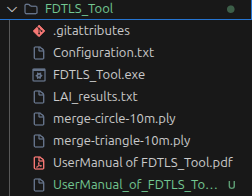
\includegraphics[width=0.45\textwidth]{fdtls.png}
    \caption{Overview of the FDTLS baseline tool.}
    \label{fig:fdtls}
\end{figure}

\section{Initial Setup and Learning Phase}
\subsection{Understanding 3DGS and Hardware}
The project began with an in-depth review of the ``3D Gaussian Splatting for Real-Time Radiance Field Rendering'' paper. Concurrently, it was crucial to learn how LiDAR sensors function and how to properly operate the FARO TLS sensor.

\subsection{Implementation Challenges}
Cloning and implementing the 3DGS repository presented significant challenges, primarily due to library dependency issues. The original 3DGS implementation relies on older versions of specific libraries, which caused version conflicts that had to be manually resolved to get the repository working correctly.

\begin{figure}[htbp]
    \centering
    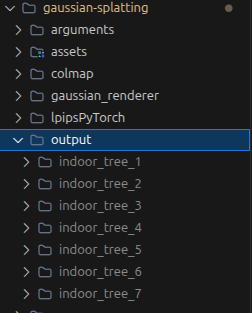
\includegraphics[width=0.45\textwidth]{making_3dgs.png}
    \caption{Process of making 3DGS.}
    \label{fig:making_3dgs}
\end{figure}

\begin{figure}[htbp]
    \centering
    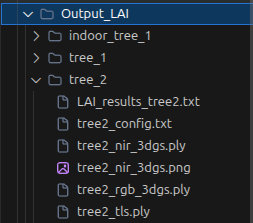
\includegraphics[width=0.45\textwidth]{making_of_lai_config_files.png}
    \caption{Making of LAI configuration files.}
    \label{fig:lai_configs}
\end{figure}

\section{Data Collection and Preprocessing}
\subsection{TLS Data Collection}
Data collection involved scanning various indoor and outdoor plants. As a first-time user of the instruments, several mistakes were made which resulted in suboptimal data:
\begin{itemize}
    \item \textbf{Distance Issues:} Placing the TLS sensor too close resulted in important parts of the plant being cut off, while placing it too far made the captured data too sparse.
    \item \textbf{Resolution Issues:} Capturing data at excessively high resolutions caused multiple crashes in the preprocessing software.
\end{itemize}

\begin{figure}[htbp]
    \centering
    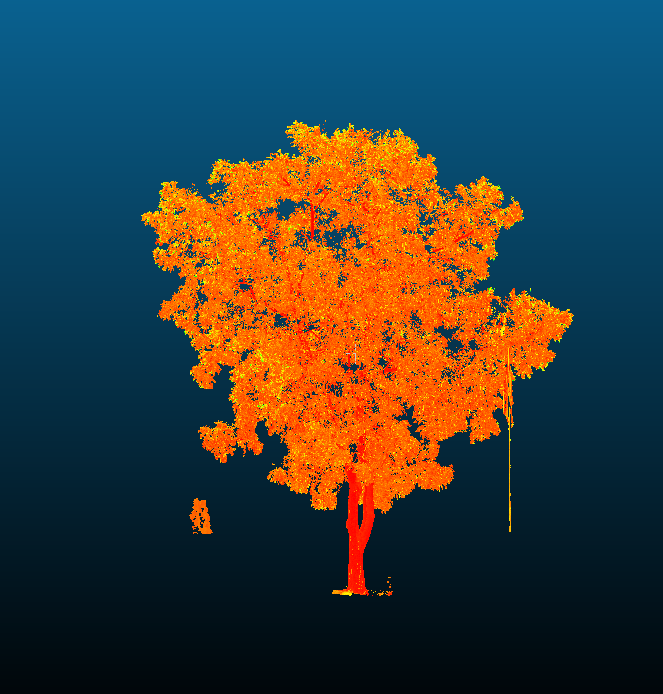
\includegraphics[width=0.45\textwidth]{tree_that_looks_dense_but_is_sparse.png}
    \caption{A tree that appears dense visually but resulted in a sparse point cloud.}
    \label{fig:sparse_tree}
\end{figure}

\begin{figure}[htbp]
    \centering
    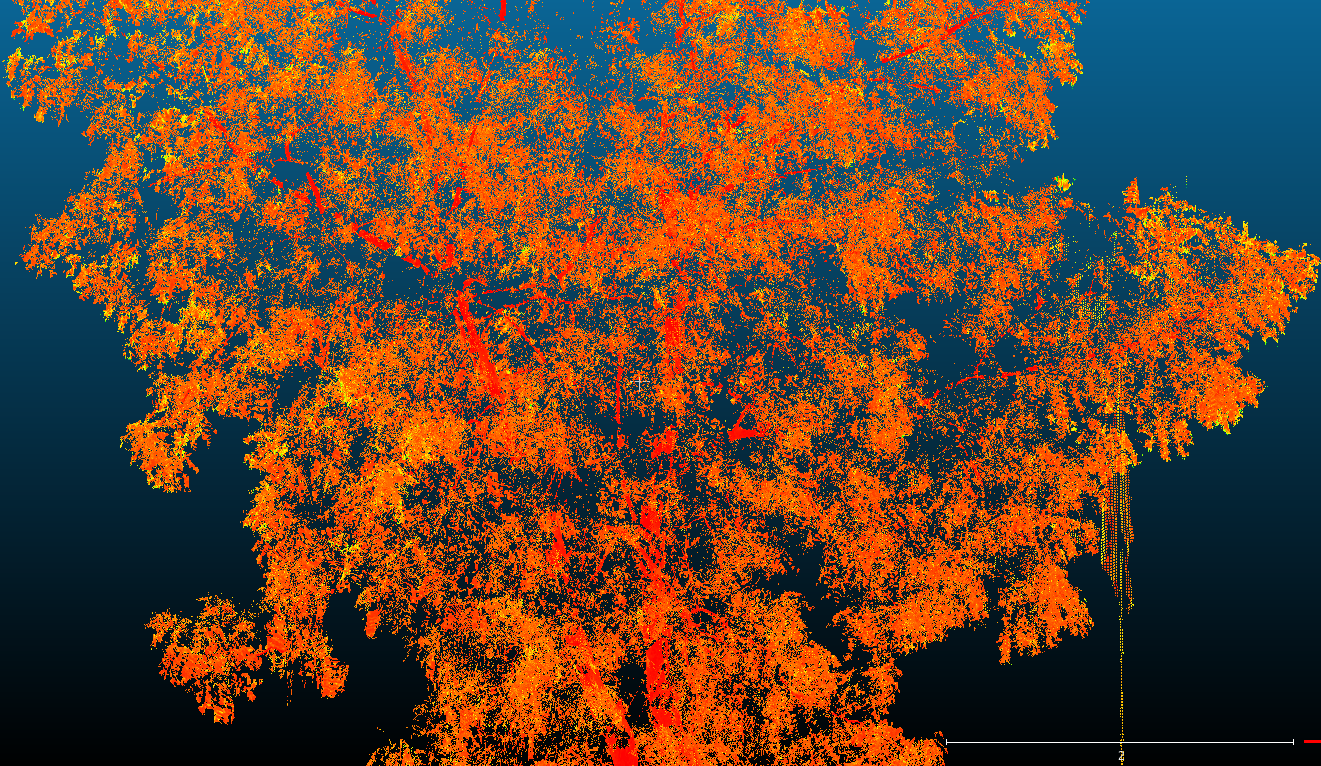
\includegraphics[width=0.45\textwidth]{sparse_tree_closeup.png}
    \caption{Close-up view of the sparse tree point cloud.}
    \label{fig:sparse_tree_closeup}
\end{figure}

\subsection{Preprocessing with FARO SCENE}
Following data collection, I learned to use the FARO SCENE preprocessing application. This software was used to preprocess and segment multiple trees from the raw TLS data.

\begin{figure}[htbp]
    \centering
    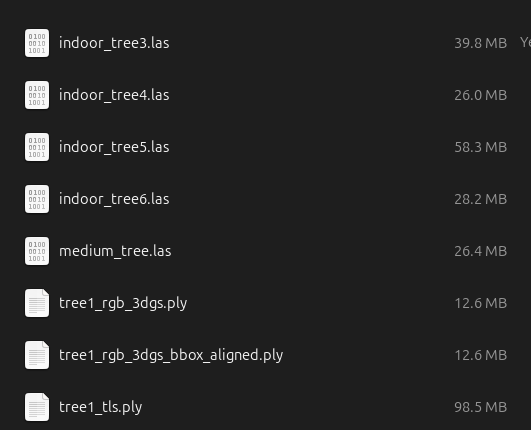
\includegraphics[width=0.45\textwidth]{preprocessing_of_tls.png}
    \caption{Preprocessing of TLS data using FARO SCENE.}
    \label{fig:preprocessing_tls}
\end{figure}

\section{3D Gaussian Splatting Generation}
\subsection{Workflow}
Videos of the plants were captured using a DJI camera to generate the 3DGS representations. The workflow is as follows:
\begin{enumerate}
    \item \textbf{Frame Extraction:} Extract frames from the input video using \texttt{ffmpeg}.
    \item \textbf{Structure from Motion:} Map these frames into a sparse point cloud using COLMAP.
    \item \textbf{Gaussian Generation:} Use \texttt{train.py} from the 3DGS repository to generate the final Gaussians.
\end{enumerate}

\begin{figure}[htbp]
    \centering
    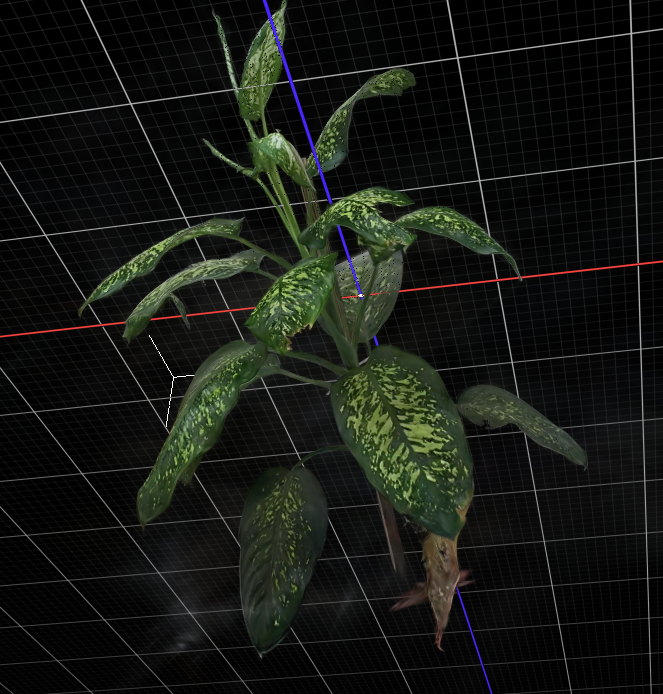
\includegraphics[width=0.45\textwidth]{3dgs_example.png}
    \caption{Example of a generated 3D Gaussian Splatting point cloud.}
    \label{fig:3dgs_example}
\end{figure}

\subsection{Issues Encountered}
Different formats were produced between the TLS and 3DGS outputs. Furthermore, I unknowingly downsampled the point clouds during the process, leading to poor results in the initial LAI estimations. After exporting \texttt{.ply} files from both TLS and 3DGS and comparing them using the FDTLS tool, the results were highly inaccurate. 

The two primary reasons for the faulty 3DGS LAI estimation were:
\begin{enumerate}
    \item \textbf{Scale Mismatch:} The TLS point cloud is in meters (world coordinate scale), while the 3DGS point cloud operates on an arbitrary scale.
    \item \textbf{Floaters in 3DGS:} Extraneous artifacts generated with no real depth.
\end{enumerate}

\section{Resolving Estimation Issues}
\subsection{Addressing Floaters}
Floaters occur because 3DGS lacks a strict sense of depth, causing it to create Gaussians out of thin air. To resolve this, I applied data post-processing on the 3DGS point cloud:
\begin{itemize}
    \item Applied an opacity filter to remove transparent Gaussians.
    \item Applied Statistical Outlier Removal (SOR) to eliminate scattered floaters.
\end{itemize}

I also researched several models designed for floater removal in 3DGS, including StableGS, GaussianFusion, and 3DGS Simplify. Using \textbf{3DGS Simplify} proved highly effective at removing floaters, although it does downsample the point cloud.

\begin{figure}[htbp]
    \centering
    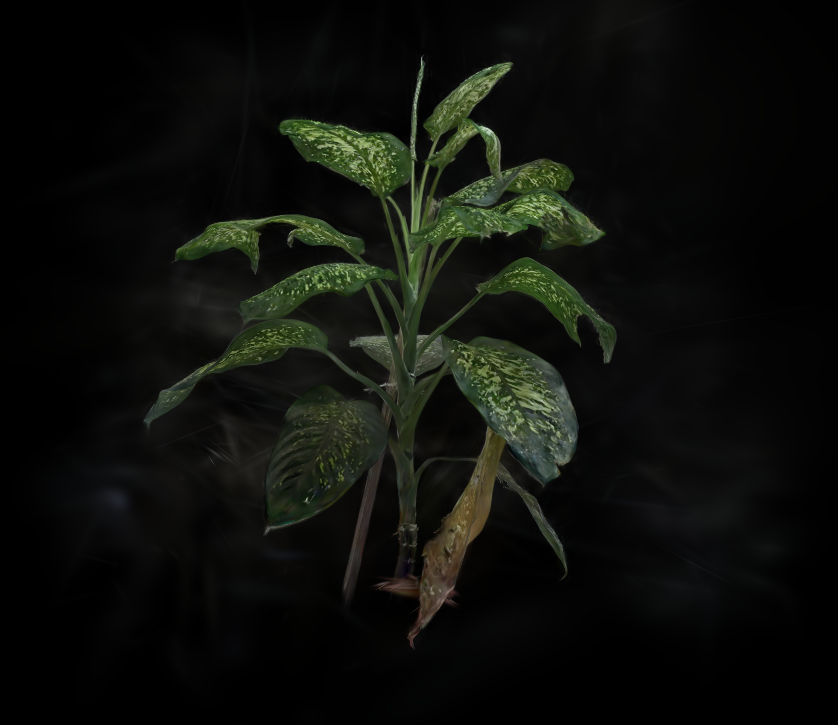
\includegraphics[width=0.45\textwidth]{3dgs_without_using_3dgs_simplify.png}
    \caption{3DGS point cloud before floater removal (showing artifacts).}
    \label{fig:3dgs_without_simplify}
\end{figure}

\begin{figure}[htbp]
    \centering
    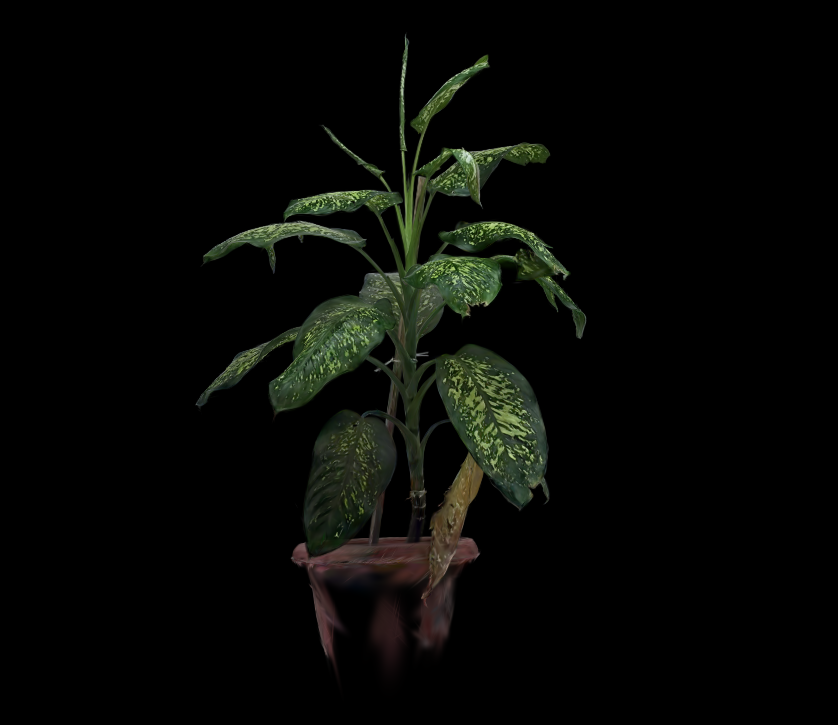
\includegraphics[width=0.45\textwidth]{3dgs_after_using_simplify.png}
    \caption{3DGS point cloud after using 3DGS Simplify for floater removal.}
    \label{fig:3dgs_after_simplify}
\end{figure}

\subsection{The Dynamic Nature of Outdoor Plants}
Another major problem during video data collection was wind causing the movement of leaves. This movement destroys the static structure assumed by 3DGS, rendering the model unusable for precise LAI estimation. Since this is a dynamic problem without an immediate solution, I shifted my focus entirely to \textbf{indoor plants}. Indoor leaves move significantly less, allowing me to isolate and tackle the scale mismatch problem first.

\section{Tackling Scale Mismatch and Point Cloud Alignment}
My most recent task has been addressing the scale mismatch to accurately overlap the 3DGS \texttt{.ply} clouds with the TLS \texttt{.ply} clouds.

\begin{figure}[htbp]
    \centering
    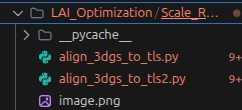
\includegraphics[width=0.45\textwidth]{scale_mismatch_fix.png}
    \caption{Visualizing the scale mismatch fix between 3DGS and TLS.}
    \label{fig:scale_mismatch_fix}
\end{figure}

\subsection{Failed Attempts at Automated Alignment}
\begin{enumerate}
    \item \textbf{Bounding Box Alignment refined by ICP:} This failed because the segmentation of the plant differed between the two point clouds.
    \item \textbf{Mapping Similar Data Point Clusters:} I attempted a pipeline using:
    \begin{itemize}
        \item Statistical Outlier Removal (SOR)
        \item DBSCAN Clustering
        \item Robust Bounding Box alignment
        \item Global Registration and Iterative Closest Point (ICP)
    \end{itemize}
    This approach also failed due to having too few correspondences after the mutual filter. Global registration relies on Fast Point Feature Histograms (FPFH), but because plants have many nearly identical leaves, the algorithm became confused and failed to establish robust feature matches.
\end{enumerate}

\begin{figure}[htbp]
    \centering
    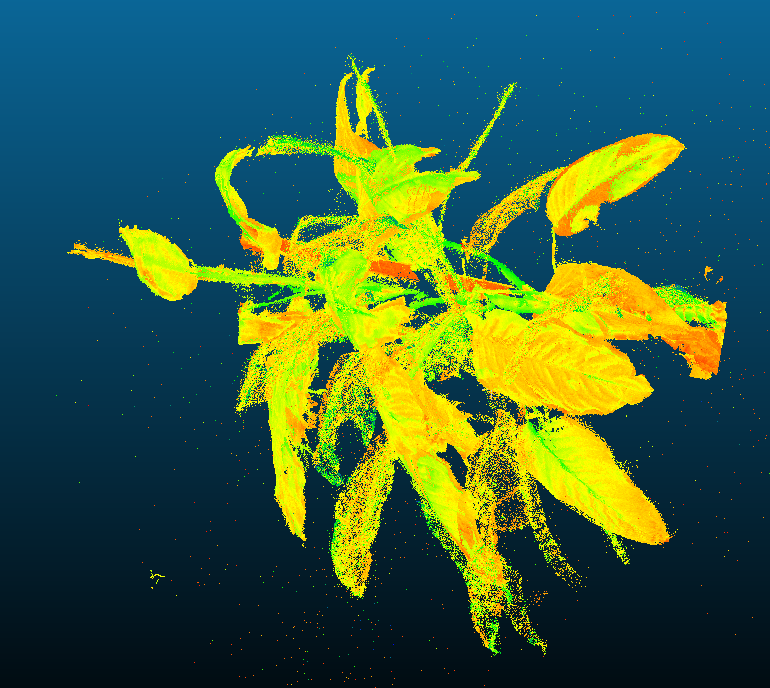
\includegraphics[width=0.45\textwidth]{auto_alignment.png}
    \caption{Attempt at automated alignment.}
    \label{fig:auto_alignment}
\end{figure}

\subsection{Successful Manual Registration}
Switching to manual registration yielded excellent results. By manually aligning the geometries, I achieved an almost perfect overlap between the 3DGS and TLS point clouds.

\begin{figure}[htbp]
    \centering
    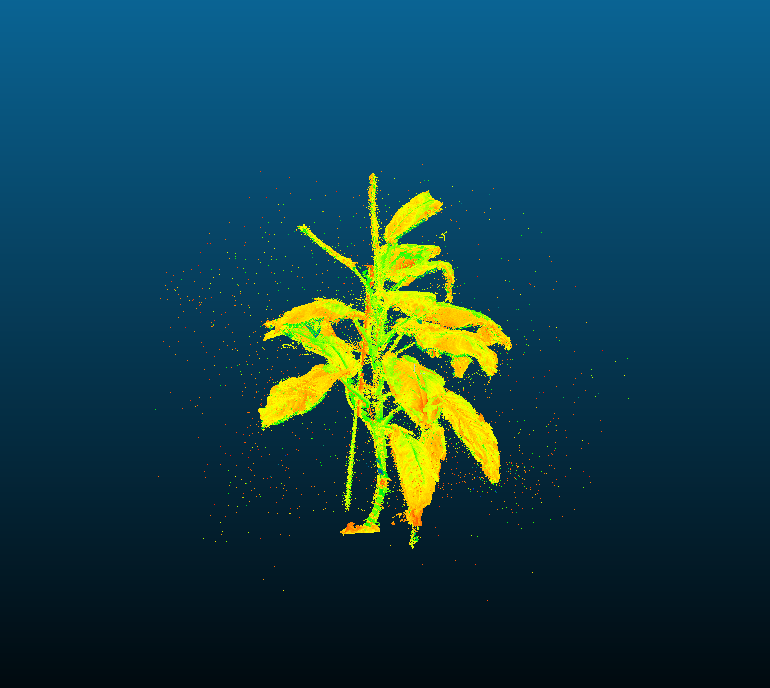
\includegraphics[width=0.45\textwidth]{perfect_alignment_by_manual.png}
    \caption{Perfect alignment achieved via manual registration.}
    \label{fig:perfect_alignment_manual}
\end{figure}

\section{Impact of Scaling on LAI Estimation}
To validate the effectiveness of the scaling process, three different indoor trees were scaled and aligned today. The LAI was then calculated and compared across three conditions for each tree: TLS (ground truth), unscaled 3DGS, and scaled (aligned) 3DGS.

The observations confirm that the scaling process is working effectively and that scale has a profound impact on LAI estimation. In all observed cases, the unscaled 3DGS point clouds consistently overestimated the LAI when compared to the TLS baseline. Once scaled properly, the LAI estimations from 3DGS aligned much more closely with the true TLS LAI values.

\begin{table}[H]
    \centering
    \begin{tabular}{|l|l|l|l|}
        \hline
        \textbf{Tree} & \textbf{Condition} & \textbf{Filename} & \textbf{LAI} \\ \hline
        \multirow{3}{*}{Tree 1} & TLS (Ground Truth) & \texttt{tree1\_tls.ply} & 0.1422 \\
        & Unscaled 3DGS & \texttt{tree1\_rgb\_3dgs.ply} & 0.2708 \\
        & Scaled 3DGS & \texttt{tree1\_rgb\_3dgs\_bbox\_aligned.ply} & 0.0906 \\ \hline
        \multirow{3}{*}{Tree 3} & TLS (Ground Truth) & \texttt{indoor\_tree3.ply} & 0.4034 \\
        & Unscaled 3DGS & \texttt{indoor\_tree3\_3dgs\_without\_pot.ply} & $2.567 \times 10^{-10}$ \\
        & Scaled 3DGS & \texttt{indoor\_tree3\_rgb\_3dgs\_bbox\_aligned.ply} & 0.4723 \\ \hline
        \multirow{3}{*}{Tree 5} & TLS (Ground Truth) & \texttt{indoor\_tree5\_wp.ply} & 0.1333 \\
        & Unscaled 3DGS & \texttt{indoor\_tree5\_3dgs\_wp.ply} & 0.3120 \\
        & Scaled 3DGS & \texttt{indoor\_tree5\_rgb\_3dgs\_bbox\_aligned.ply} & 0.0664 \\ \hline
    \end{tabular}
    \caption{LAI calculation results comparing TLS, unscaled 3DGS, and scaled 3DGS across three indoor trees.}
    \label{tab:results_three_trees}
\end{table}

\subsection{Tree 3 Analysis}
\begin{figure}[htbp]
    \centering
    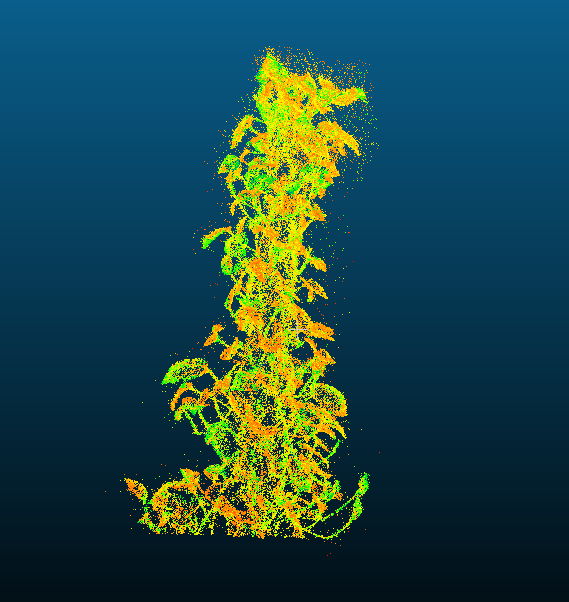
\includegraphics[width=0.45\textwidth]{indoor_tree3_tls.png}
    \caption{TLS point cloud for Indoor Tree 3.}
    \label{fig:tree3_tls}
\end{figure}

\begin{figure}[htbp]
    \centering
    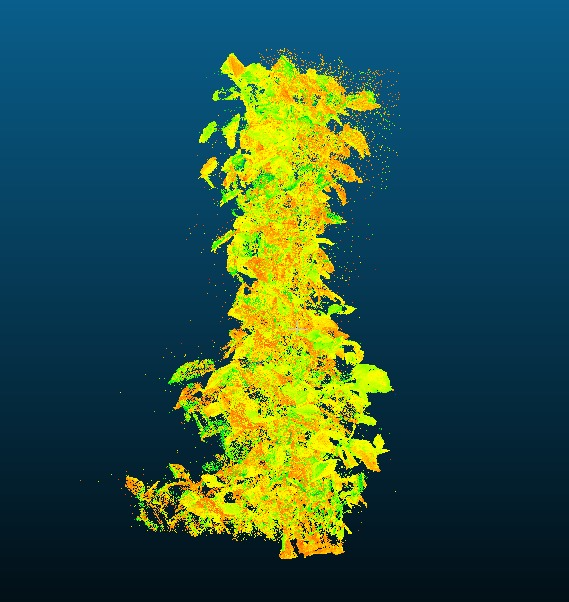
\includegraphics[width=0.45\textwidth]{tree3_scaled_to_the_same_size.png}
    \caption{Tree 3 3DGS point cloud scaled to match the TLS size.}
    \label{fig:tree3_scaled}
\end{figure}

\begin{figure}[htbp]
    \centering
    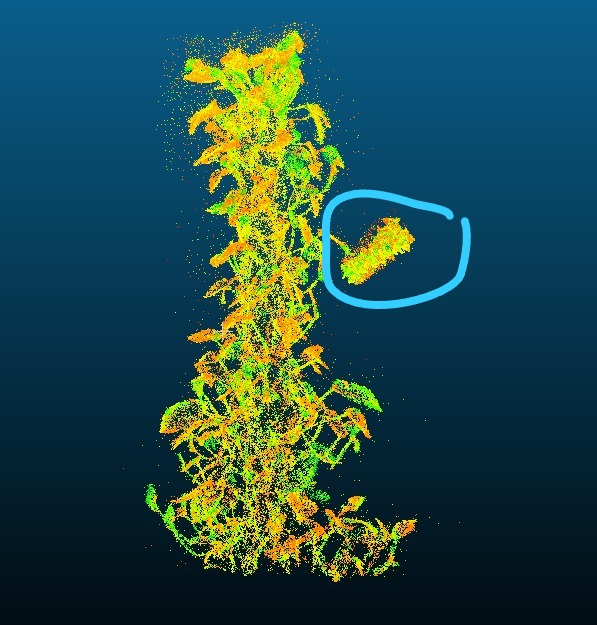
\includegraphics[width=0.45\textwidth]{indoor_tree3_scaledvsunscaled_comparison.png}
    \caption{Comparison of scaled vs. unscaled 3DGS for Indoor Tree 3.}
    \label{fig:tree3_comparison}
\end{figure}

\subsection{Tree 5 Analysis}
\begin{figure}[htbp]
    \centering
    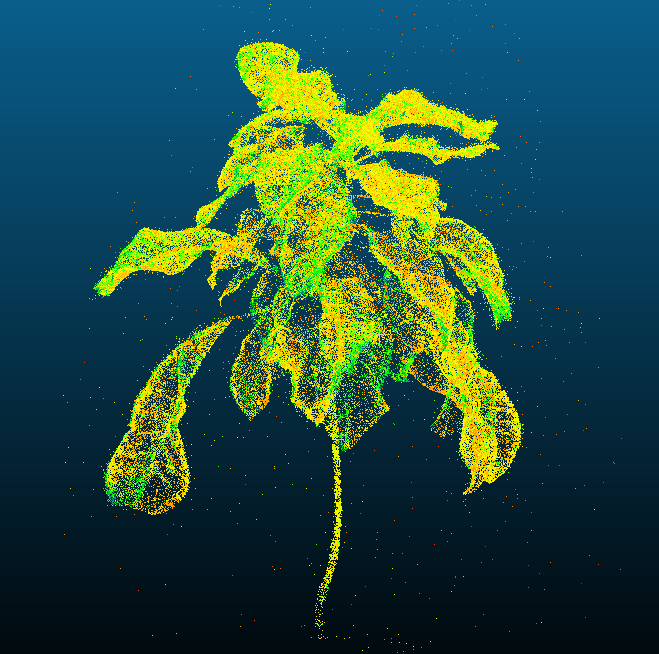
\includegraphics[width=0.45\textwidth]{indoor_tree5_3dgs.png}
    \caption{Unscaled 3DGS point cloud for Indoor Tree 5.}
    \label{fig:tree5_3dgs}
\end{figure}

\begin{figure}[htbp]
    \centering
    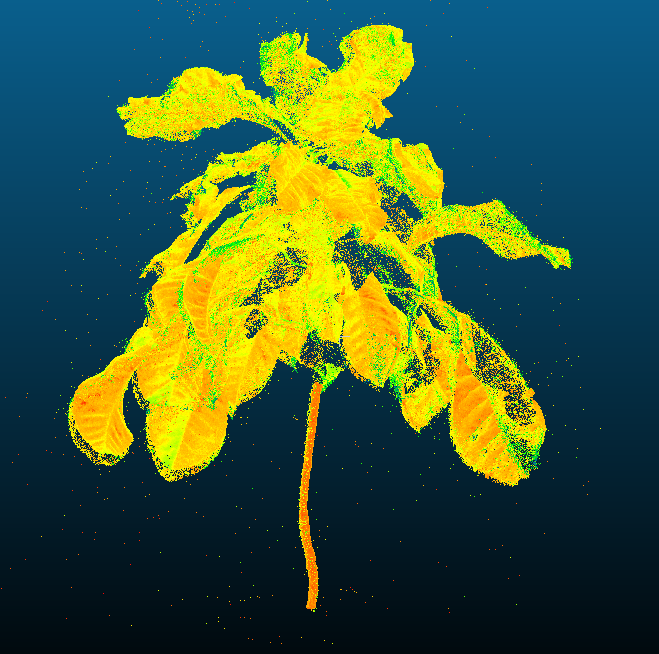
\includegraphics[width=0.45\textwidth]{indoor_tree5_scaled_overlapping_properly.png}
    \caption{Indoor Tree 5 scaled 3DGS overlapping properly with the TLS reference.}
    \label{fig:tree5_overlap}
\end{figure}

\begin{figure}[htbp]
    \centering
    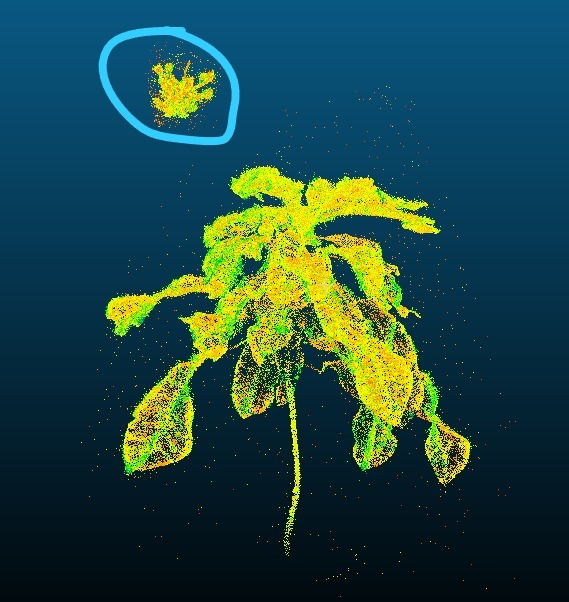
\includegraphics[width=0.45\textwidth]{indoor_tree5_scaledvsunscaled_comparison.png}
    \caption{Comparison of scaled vs. unscaled 3DGS for Indoor Tree 5.}
    \label{fig:tree5_comparison}
\end{figure}

\section{Automated Alignment Pipeline (PCA-ICP)}
To overcome the limitations of manual alignment and the failures of global registration, a fully automated pipeline was developed. This pipeline successfully regularizes the scale and aligns the 3DGS point clouds to the metric TLS reference without human intervention. The pipeline consists of:
\begin{enumerate}
    \item \textbf{Voxel Downsampling \& SOR:} Standardizing point density and removing isolated noise.
    \item \textbf{DBSCAN Clustering:} Extracting the primary plant structure and discarding large floaters.
    \item \textbf{PCA Scale Estimation:} Automatically estimating the isotropic scale factor using the median ratio of the PCA standard deviations from both point clouds.
    \item \textbf{Z-Rotation Sweep \& ICP:} Testing all 180-degree eigenvector flips and refining them using Point-to-Plane Iterative Closest Point (ICP). The best fit is selected using a composite score (Fitness / RMSE).
\end{enumerate}

This automated pipeline works flawlessly, achieving F-scores of 99.08\% for the Outdoor Small Plant and 99.84\% for Tree 5 (after post-processing).

\section{Post-Processing Ablation and LAI Correlation}
Following the automated alignment, post-processing (SOR) was applied to remove remaining floaters. Calculating the FDTLS LAI on these auto-aligned and post-processed clouds revealed a highly consistent and scientifically reassuring trend: \textbf{structural point-cloud geometry and ecological metric accuracy are tightly correlated}.

\begin{itemize}
    \item For datasets where floaters were safely removed without destroying the canopy (e.g., Tree 5 and Outdoor Small Plant), the geometric F-score improved, and the relative LAI error dropped massively (e.g., Tree 5 LAI error dropped from 38.18\% to 5.33\%).
    \item Conversely, for datasets where the filtering was too aggressive and accidentally removed legitimate thin canopy structures (e.g., Tree 1 and Bushes), the geometric F-score worsened, and consequently, the LAI error worsened.
\end{itemize}

This proves that FDTLS is highly sensitive to physical occupancy, and accurate LAI estimation strictly requires high-fidelity, scale-accurate geometric reconstruction.

\begin{table}[H]
    \centering
    \renewcommand{\arraystretch}{1.3}
    \resizebox{\columnwidth}{!}{
    \begin{tabular}{|l|c|c|c|c|}
        \hline
        \textbf{Dataset} & \textbf{TLS LAI} & \textbf{Scaled 3DGS LAI} & \textbf{Post-processed 3DGS LAI} & \textbf{Final Error (\%)} \\ \hline
        Bushes & 0.5656 & 0.6455 & 0.6725 & 18.90\% \\ \hline
        Outdoor Small Plant & 0.4091 & 0.5210 & 0.4660 & 13.91\% \\ \hline
        Tree 1 & 0.1422 & 0.2099 & 0.0683 & 51.97\% \\ \hline
        Tree 5 & 0.1333 & 0.0824 & 0.1262 & 5.33\% \\ \hline
    \end{tabular}
    }
    \caption{Final LAI estimations using the automated pipeline.}
    \label{tab:final_lai}
\end{table}

\section{Next Steps}
With the automated scaling and alignment challenges successfully solved, future tasks include:
\begin{itemize}
    \item Identifying state-of-the-art (SOTA) baseline models for:
    \begin{itemize}
        \item Biomass estimation
        \item Urban carbon accounting
        \item Urban canopy estimation
    \end{itemize}
    \item Resuming data collection for outdoor plants, specifically bushes, medium trees, and large trees, once dynamic wind-induced movement challenges are better understood.
\end{itemize}

\end{document}
